\section{Pixels}
\begin{minipage}{0.5\textwidth}
%\subsection*{Agenda}
\begin{enumerate}
\item How to draw a staright'ish line
\end{enumerate}
\end{minipage}
\begin{minipage}{0.5\textwidth}
\begin{center}
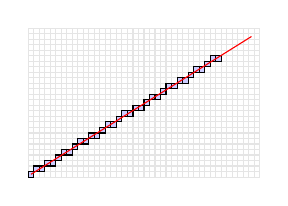
\begin{tikzpicture}[scale=0.07]
\draw[ black!10!white] (0,0) grid (42,27);
%\foreach \x in {0,1,2,...,13}{\draw[] ({\x+0.5}, -0.5) node[] {$\x$}; }
%\foreach \y in {0,1,2,...,8}{\draw[] (-0.5,{\y+0.5}) node[] {$\y$}; }

%\draw[->] (0,0) -- (14,0);% node[right]{$\Delta m$};
%\draw[->] (0,0) -- (0,9);% node[above]{$\Delta x $};
%

\foreach \x in {0}{ \foreach \y in {0}{  
\filldraw[fill=blue!20!white, draw=black] (\x,\y) rectangle ({\x+1},{\y+1});}}

\foreach \x in {1,2}{ \foreach \y in {1}{  
\filldraw[fill=blue!20!white, draw=black] (\x,\y) rectangle ({\x+1},{\y+1});}}

\foreach \x in {3,4}{ \foreach \y in {2}{  
\filldraw[fill=blue!20!white, draw=black] (\x,\y) rectangle ({\x+1},{\y+1});}}

\foreach \x in {5}{ \foreach \y in {3}{  
\filldraw[fill=blue!20!white, draw=black] (\x,\y) rectangle ({\x+1},{\y+1});}}

\foreach \x in {6,7}{ \foreach \y in {4}{  
\filldraw[fill=blue!20!white, draw=black] (\x,\y) rectangle ({\x+1},{\y+1});}}

\foreach \x in {8}{ \foreach \y in {5}{  
\filldraw[fill=blue!20!white, draw=black] (\x,\y) rectangle ({\x+1},{\y+1});}}

\foreach \x in {9,10}{ \foreach \y in {6}{  
\filldraw[fill=blue!20!white, draw=black] (\x,\y) rectangle ({\x+1},{\y+1});}}

\foreach \x in {11,12}{ \foreach \y in {7}{  
\filldraw[fill=blue!20!white, draw=black] (\x,\y) rectangle ({\x+1},{\y+1});}}

\foreach \x in {13}{ \foreach \y in {8}{  
\filldraw[fill=blue!20!white, draw=black] (\x,\y) rectangle ({\x+1},{\y+1});}}




\foreach \x in {14,15}{ \foreach \y in {9}{  
\filldraw[fill=blue!20!white, draw=black] (\x,\y) rectangle ({\x+1},{\y+1});}}

\foreach \x in {16}{ \foreach \y in {10}{  
\filldraw[fill=blue!20!white, draw=black] (\x,\y) rectangle ({\x+1},{\y+1});}}

\foreach \x in {17,18}{ \foreach \y in {11}{  
\filldraw[fill=blue!20!white, draw=black] (\x,\y) rectangle ({\x+1},{\y+1});}}

\foreach \x in {19,20}{ \foreach \y in {12}{  
\filldraw[fill=blue!20!white, draw=black] (\x,\y) rectangle ({\x+1},{\y+1});}}

\foreach \x in {21}{ \foreach \y in {13}{  
\filldraw[fill=blue!20!white, draw=black] (\x,\y) rectangle ({\x+1},{\y+1});}}

\foreach \x in {22,23}{ \foreach \y in {14}{  
\filldraw[fill=blue!20!white, draw=black] (\x,\y) rectangle ({\x+1},{\y+1});}}

\foreach \x in {24}{ \foreach \y in {15}{  
\filldraw[fill=blue!20!white, draw=black] (\x,\y) rectangle ({\x+1},{\y+1});}}




\foreach \x in {25,26}{ \foreach \y in {16}{  
\filldraw[fill=blue!20!white, draw=black] (\x,\y) rectangle ({\x+1},{\y+1});}}

\foreach \x in {27,28}{ \foreach \y in {17}{  
\filldraw[fill=blue!20!white, draw=black] (\x,\y) rectangle ({\x+1},{\y+1});}}

\foreach \x in {29}{ \foreach \y in {18}{  
\filldraw[fill=blue!20!white, draw=black] (\x,\y) rectangle ({\x+1},{\y+1});}}

\foreach \x in {30,31}{ \foreach \y in {19}{  
\filldraw[fill=blue!20!white, draw=black] (\x,\y) rectangle ({\x+1},{\y+1});}}

\foreach \x in {32}{ \foreach \y in {20}{  
\filldraw[fill=blue!20!white, draw=black] (\x,\y) rectangle ({\x+1},{\y+1});}}

\foreach \x in {33,34}{ \foreach \y in {21}{  
\filldraw[fill=blue!20!white, draw=black] (\x,\y) rectangle ({\x+1},{\y+1});}}


%\foreach \x in {0,1,2,...,13}{ \foreach \y in {0,1,2,...,8}{  
%\pgfmathparse{int((8*\x)-(13*\y))} \let\n\pgfmathresult
% \draw[black] ({\x},{\y}) node[above,xshift=10pt] {$\n$};}}
 
\draw[ red] (0.5,0.5) -- ({3*13.5},{3*8.5});
\end{tikzpicture}
\end{center}
\end{minipage}

\vspace{2em}




Fill in the squares that you think make for the best line from $(0,0)$ to $(13,8)$

\begin{center}
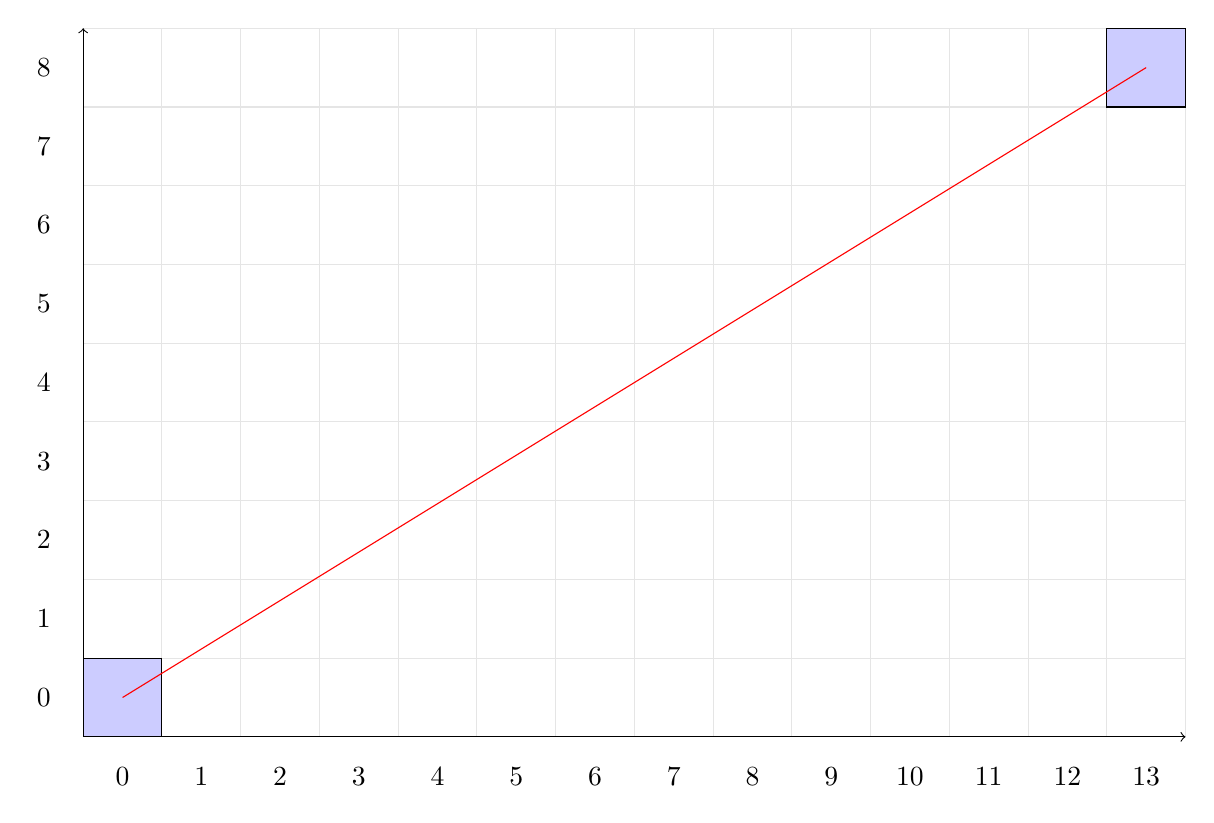
\begin{tikzpicture}[scale=1]
\draw[ black!10!white] (0,0) grid (14,9);
\foreach \x in {0,1,2,...,13}{\draw[] ({\x+0.5}, -0.5) node[] {$\x$}; }
\foreach \y in {0,1,2,...,8}{\draw[] (-0.5,{\y+0.5}) node[] {$\y$}; }

\draw[->] (0,0) -- (14,0);% node[right]{$\Delta m$};
\draw[->] (0,0) -- (0,9);% node[above]{$\Delta x $};


\foreach \x in {0}{ \foreach \y in {0}{  
\filldraw[fill=blue!20!white, draw=black] (\x,\y) rectangle ({\x+1},{\y+1});}}

%\foreach \x in {1,2}{ \foreach \y in {1}{  
%\filldraw[fill=blue!20!white, draw=black] (\x,\y) rectangle ({\x+1},{\y+1});}}
%
%\foreach \x in {3,4}{ \foreach \y in {2}{  
%\filldraw[fill=blue!20!white, draw=black] (\x,\y) rectangle ({\x+1},{\y+1});}}
%
%\foreach \x in {5}{ \foreach \y in {3}{  
%\filldraw[fill=blue!20!white, draw=black] (\x,\y) rectangle ({\x+1},{\y+1});}}
%
%\foreach \x in {6,7}{ \foreach \y in {4}{  
%\filldraw[fill=blue!20!white, draw=black] (\x,\y) rectangle ({\x+1},{\y+1});}}
%
%\foreach \x in {8}{ \foreach \y in {5}{  
%\filldraw[fill=blue!20!white, draw=black] (\x,\y) rectangle ({\x+1},{\y+1});}}
%
%\foreach \x in {9,10}{ \foreach \y in {6}{  
%\filldraw[fill=blue!20!white, draw=black] (\x,\y) rectangle ({\x+1},{\y+1});}}
%
%\foreach \x in {11,12}{ \foreach \y in {7}{  
%\filldraw[fill=blue!20!white, draw=black] (\x,\y) rectangle ({\x+1},{\y+1});}}

\foreach \x in {13}{ \foreach \y in {8}{  
\filldraw[fill=blue!20!white, draw=black] (\x,\y) rectangle ({\x+1},{\y+1});}}

%\foreach \x in {0,1,2,...,13}{ \foreach \y in {0,1,2,...,8}{  
%\pgfmathparse{int((8*\x)-(13*\y))} \let\n\pgfmathresult
% \draw[black] ({\x},{\y}) node[above,xshift=10pt] {\small$\n$};}}
 
\draw[ red] (0.5,0.5) -- (13.5,8.5);
\end{tikzpicture}

\end{center}



Identify the parts $D$ and $D_{vert}$ and observe that optimizing one implies optimizing the other.

\begin{minipage}{0.5\textwidth}
\notes{10}
\end{minipage}
\begin{minipage}{0.5\textwidth}
\begin{center}
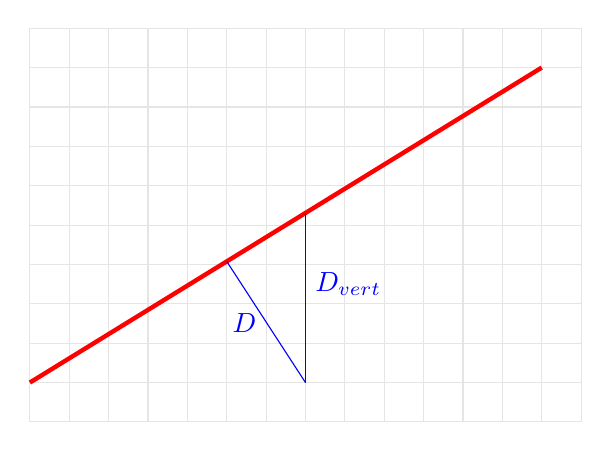
\begin{tikzpicture}[scale=0.5]
\draw[ black!10!white] (0,-1) grid (14,9);
\draw[ultra thick, red] (0,0) -- (13,8);
\draw[ blue] (7, 0.615*7) -- (7,0) ;
\draw[ blue] (7,0) -- (	5 ,8/13*5);
\draw[ blue]  (7,2.5) node[right] {$D_{vert}$};
\draw[ blue] (6,1.5) node[left] {$D$};
\end{tikzpicture} 
\end{center}
\end{minipage}

\newpage
%\begin{minipage}{0.5\textwidth}
\begin{center}
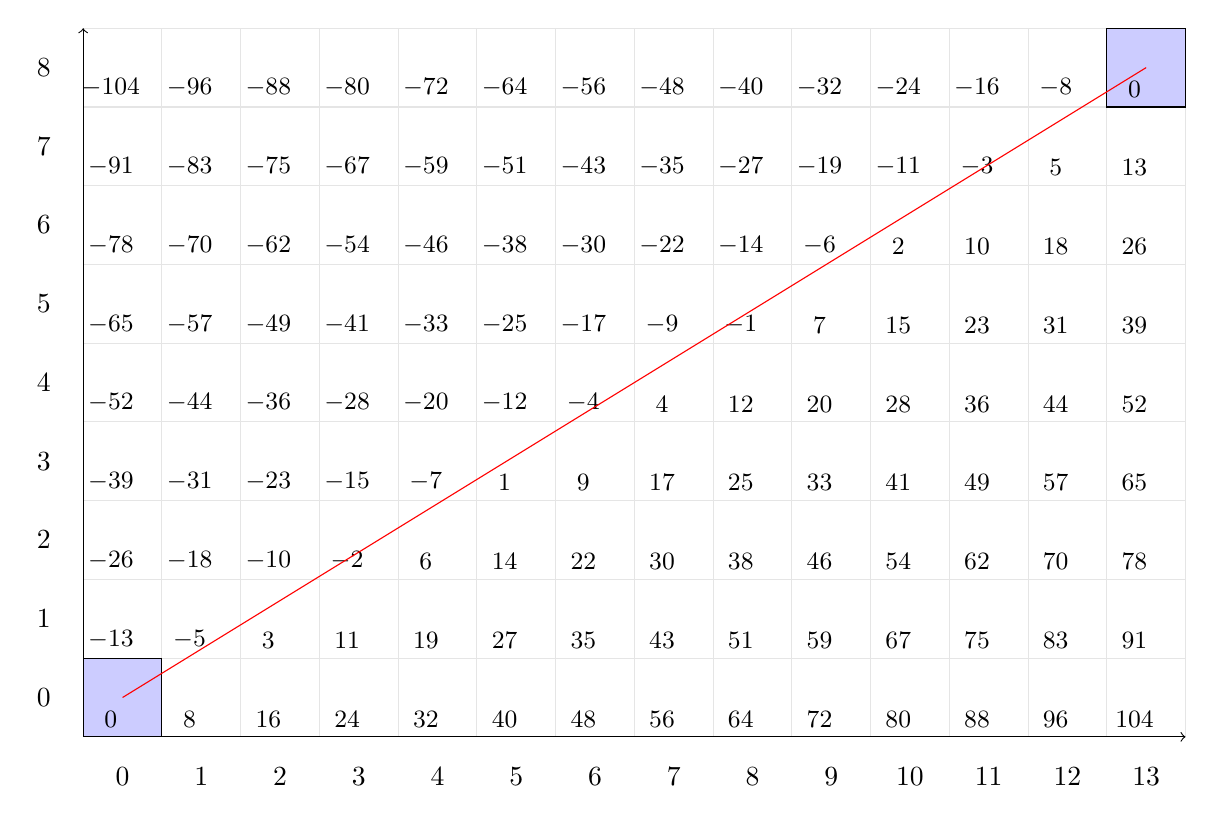
\begin{tikzpicture}[scale=1]
\draw[ black!10!white] (0,0) grid (14,9);
\foreach \x in {0,1,2,...,13}{\draw[] ({\x+0.5}, -0.5) node[] {$\x$}; }
\foreach \y in {0,1,2,...,8}{\draw[] (-0.5,{\y+0.5}) node[] {$\y$}; }

\draw[->] (0,0) -- (14,0);% node[right]{$\Delta m$};
\draw[->] (0,0) -- (0,9);% node[above]{$\Delta x $};


\foreach \x in {0}{ \foreach \y in {0}{  
\filldraw[fill=blue!20!white, draw=black] (\x,\y) rectangle ({\x+1},{\y+1});}}

%\foreach \x in {1,2}{ \foreach \y in {1}{  
%\filldraw[fill=blue!20!white, draw=black] (\x,\y) rectangle ({\x+1},{\y+1});}}
%
%\foreach \x in {3,4}{ \foreach \y in {2}{  
%\filldraw[fill=blue!20!white, draw=black] (\x,\y) rectangle ({\x+1},{\y+1});}}
%
%\foreach \x in {5}{ \foreach \y in {3}{  
%\filldraw[fill=blue!20!white, draw=black] (\x,\y) rectangle ({\x+1},{\y+1});}}
%
%\foreach \x in {6,7}{ \foreach \y in {4}{  
%\filldraw[fill=blue!20!white, draw=black] (\x,\y) rectangle ({\x+1},{\y+1});}}
%
%\foreach \x in {8}{ \foreach \y in {5}{  
%\filldraw[fill=blue!20!white, draw=black] (\x,\y) rectangle ({\x+1},{\y+1});}}
%
%\foreach \x in {9,10}{ \foreach \y in {6}{  
%\filldraw[fill=blue!20!white, draw=black] (\x,\y) rectangle ({\x+1},{\y+1});}}
%
%\foreach \x in {11,12}{ \foreach \y in {7}{  
%\filldraw[fill=blue!20!white, draw=black] (\x,\y) rectangle ({\x+1},{\y+1});}}

\foreach \x in {13}{ \foreach \y in {8}{  
\filldraw[fill=blue!20!white, draw=black] (\x,\y) rectangle ({\x+1},{\y+1});}}

\foreach \x in {0,1,2,...,13}{ \foreach \y in {0,1,2,...,8}{  
\pgfmathparse{int((8*\x)-(13*\y))} \let\n\pgfmathresult
 \draw[black] ({\x},{\y}) node[above,xshift=10pt] {\small$\n$};}}
 
\draw[ red] (0.5,0.5) -- (13.5,8.5);
\end{tikzpicture}

\end{center}
%\end{minipage}

\notes{15}




 
 